\documentclass{article}
\usepackage{graphicx} % Required for inserting images
\usepackage{amsmath}
\usepackage{threeparttable}
\usepackage[margin=1in]{geometry}
\usepackage{setspace}
\doublespacing
\setlength{\parskip}{1em}
\setlength{\parindent}{0pt}
\usepackage[authordate, backend=biber]{biblatex-chicago}
\addbibresource{../references.bib}
\usepackage[bottom]{footmisc}

\usepackage{float}
\usepackage{etoolbox}
\AtBeginEnvironment{table}{\singlespacing}
\AtBeginEnvironment{longtable}{\singlespacing}

% abstract stuff
\AtBeginEnvironment{abstract}{\singlespacing}
\makeatletter
\renewenvironment{abstract}{\small\quotation}{\endquotation}
\makeatother

\usepackage{multirow}
\usepackage{caption}
\usepackage{longtable}
\captionsetup[table]{skip=8pt}
\usepackage{hyperref}
\title{Do Stronger Trade Ties Mitigate Tariff Shocks? Evidence from 2018 US Tariffs}
\author{Elek Krizsán\thanks{George Washington University, Department of Economics \& Elliott School of International Affairs. Contact: elekkrizsan@gwu.edu; elekkrizsan@gmail.com. Acknowledgements: I thank Professor Tara Sinclair and Chesapeake Dowdy for guidance throughout this project, as well as Professor Tomas Williams, Professor Maggie Chen, Adrian Torres-Trigo, Cage Englander, Adam Benko-Badr, Vidya Shah, Ria Saxena, Francisco Rotman, Devika Mukherjee, Mish Quan, Natalie Arbatman, and Satya Vangoor for helpful comments and suggestions. I also express appreciation to Anthropic for developing Claude, which has been a valuable thinking partner. I am grateful to Amiti, Redding, and Weinstein for making their data and replication code publicly available. All remaining errors are my own.}}
\date{May 2026}

\begin{document}

    \maketitle

    \begin{abstract}
The 2018--2019 US trade war arrived after decades of efforts to deepen global economic ties through trade agreements, raising the question of whether these institutionalized relationships make countries more resilient to sudden, unilateral tariff shocks. This paper studies whether countries with bilateral trade agreements with the United States experienced different effects of tariffs on prices and volumes than countries without such agreements. Extending the event-study framework of Amiti, Redding, and Weinstein (2020), I construct a triple-differences design using monthly customs data at the country-product level, restricting attention to the first three tariff waves (Section 201 and Section 232) which applied non-discriminatorily across countries. I find that import volumes from agreement countries rose following tariff implementation while volumes from non-agreement countries fell: a 25\% tariff is associated with an approximately 25\% rise in imports from agreement countries and an approximately 44\% decline in imports from non-agreement countries twelve months after implementation. This effect is concentrated in steel products, where the volume gain for agreement countries is large and persistent; non-steel agreement countries experience only a transient volume gain that reverses after roughly six months, indicating that the resilience effect operates differently across product categories. The price evidence is consistent with the volume findings but cannot be causally identified due to pre-trend violations within product subsamples. These patterns are consistent with a cost-buffer mechanism in which prior tariff and non-tariff barrier reductions under existing agreements leave agreement-country exporters better positioned to absorb tariff shocks, complemented by expectations-based channels through which importers rebalance toward partners with more predictable policy environments.
\end{abstract}

    \clearpage

    \section{Introduction}

In February 2018, after decades of globalization and economic integration, the Trump Administration imposed the first of eight major waves of tariffs targeting both China and other trading partners across a variety of goods, initiating the first of two trade wars. These raised the cost of trade for countries exporting to the United States, though numerous studies have found that tariff costs were passed entirely onto US consumers \autocite{fajgelbaumEconomicImpactsUS2022}. Tariffs also both substantially and persistently reduced trade volumes \autocite{amiti_whos_2020}. These findings imply that tariffs are a force of economic disintegration, where prices are higher when we trade, and so we trade less. Yet this trade war arrived in the wake of decades of efforts to deepen global economic ties. This paper asks whether those efforts were in vain. It asks whether the hallmark of integration --- the free trade agreement --- which over the decades has moved beyond a tool to reduce tariffs and increasingly into policy tools to reduce other barriers to trade \autocite{hofmann2017}, helps countries weather the storms trade wars incite. It asks whether deeper trade agreements made countries more resilient to the repeated unilateral tariff shock that was the 2018 trade war. 

The primary consequences of tariffs, the literature finds, were higher prices and less trade. Many studies have found complete pass-through of tariffs to prices paid by importers at the border \autocite{amiti_whos_2020, fajgelbaum2020, cavalloTariffPassThroughBorder2021}, meaning that foreign firms raise prices by exactly the tariff amount, forcing US firms to bear their cost entirely. Interestingly, this is inconsistent with international trade theory, which has long posited that tariffs imposed by a large country would result in incomplete pass-through due to its market power in the global economy \autocite{fajgelbaumEconomicImpactsUS2022}. To retain access to the country's large market, global exporters would reduce their prices, thus absorbing some of the tariff costs. Empirical evidence supported this, consistently finding incomplete pass-through.\footnote{For a more detailed review of tariff pass-through in general and due to the 2018 trade war, see \autocite{fajgelbaumEconomicImpactsUS2022} section 4.1.} Meanwhile, tariffs also reduced trade volumes, defined as the dollar value of imports in a given period \autocite{fajgelbaum2020, amiti2019_tariffs, amiti_whos_2020}. This more closely reflects traditional international trade theory, which predicts tariffs will lower export volumes to the tariffing country. 

Deep trade agreements --- defined as trade agreements that cover more policy areas --- have been shown to lead to higher trade. Deep trade agreements reduce both tariff and non-tariff barriers to trade. The first objective of trade agreements has historically been to reduce tariffs beyond WTO requirements --- tariff reductions are the most common provision in trade agreements, while non-tariff policy provisions vary to a greater degree \autocite{hofmann2017}. Reductions in non-tariff barriers through deep trade agreements have been shown to lead to higher trade creation while causing less trade diversion \autocite{mattooTradeCreationTrade2022}. Greater trade creation, or increased trade between trade agreement members, is a result of discriminatory policies within agreements that affect only those countries who are party to the agreement (e.g. preferential access, mutual recognition, or regulatory alignment). Reduced trade diversion means that deeper agreements reduce the likelihood that agreement members substitute each others' goods for products previously imported from non-members. These are a result of non-discriminatory policies (e.g. competition policy or customs improvements) that apply to all trade relationships. Finally, trade agreements reduce uncertainty \autocite{TPU_literature_review, carballo2022}.\footnote{For further literature on the economic impacts of deep trade agreements, see the literature review by \textcite{fernandes2021}.} These four factors --- reduced tariffs, discriminatory and non-discriminatory policies, and reduced uncertainty --- not only increase trade, but typically reduce costs in the long run. Three of the four factors, excluding only non-discriminatory policies, affect only agreement partners. Under this framework and under conditions of established agreements (where adjustment costs due to factors like regulatory alignment have already been incurred and overcome), I predict that agreement participants have relatively lower trade costs compared to non-participants, creating a wedge between these groups' trade costs. Therefore, in the case of a unilaterally-imposed tariff shock, this wedge helps firms from countries that share bilateral trade agreements with the US to more easily absorb tariff costs, leading to lower pass-through. Meanwhile, I predict that reduced uncertainty and enhanced price competitiveness under these conditions would also lead to a smaller decline in trade volumes.

As such, this paper poses the following question: did the effect of tariffs on countries' trade with the United States differ depending on the depth of countries' trade agreements with the US? In doing so, it asks whether more institutionalized trade relationships are more resilient to trade disruptions as a result of protectionism. It contributes to two main strands of the literature. First, it extends the literature on tariffs' welfare impacts, exploring heterogeneities in tariffs' effects. Understanding how tariffs affect different groups, products, and industries is important to designing effective trade policy. Second, it contributes a new perspective on trade agreements as resilience-enhancing tools, which is all the more important in today's world of geoeconomic instability and unpredictability. As countries like the EU seek to use trade agreements to diversify and institutionalize their trade relationships, understanding trade agreements' diverse impacts can help design agreements more aligned with policy objectives. 

This paper studies whether trade agreements do indeed lead to lower pass-through and lower volume reduction. Extending \textcite{amiti_whos_2020}, I construct an event-study framework with a triple-differences interpretation that identifies the differential effect of trade agreements on prices and volumes.\footnote{For a formalization of the triple-difference estimator, see \textcite{oldenTripleDifferenceEstimator2022}.} I examine the differential effect of agreements on two outcome variables, prices and volumes, examining the first three waves of tariffs. These were imposed through Section 201 and 232 tariffs, applying non-discriminatorily across all countries importing solar panels, washing machines, steel products, and aluminum products. It turns out the US's 20 trade agreements are all primarily deep, meaning there is no sufficient sample of shallow trade agreements to compare their effect to. As such, the paper proceeds with studying the differential effects of trade agreements in general with respect to prices and volumes following exposure to tariffs. 

My results find that countries with bilateral US trade agreements were more resilient to the 2018 tariff shock than countries without. Following tariff implementation, import volumes from agreement countries rose while volumes from non-agreement countries fell, suggesting that institutionalized trade relationships moderated the impact of unilateral tariffs. This aggregate effect is driven by steel products and exhibits a similar but short-lived trend for non-steel products, indicating that the resilience-enhancing role of trade agreements may operate differently depending on product characteristics. The price evidence is consistent with this pattern but cannot be causally identified due to pre-trend violations within product subsamples. These patterns are consistent with the cost-buffer mechanism developed in this paper, in which prior tariff and non-tariff barrier reductions leave agreement-country exporters better positioned to absorb tariff shocks.

The remainder of this paper is organized as follows. Section~\ref{sec:data} describes the data sources and presents descriptive statistics on tariffs, trade agreements, and trade flows. Section~\ref{sec:models} walks through a model to calibrate the restricted sample with the foundational paper, the main triple-difference model, and an examination of heterogeneity between steel and non-steel products due to the high share of the sample constituted by steel products. Section~\ref{sec:results} describes trade agreements' differential price and volume elasticities with respect to tariffs, and Section~\ref{sec:discussion} interprets results, highlighting data issues and assumption violations, along with a discussion of limitations and avenues for future research. Finally, Section~\ref{sec:conclusion} concludes. 



    \section{Data}\label{sec:data}

\subsection{Dataset construction}

To construct price and volume variables I use monthly US customs data from the US Census Bureau between January 2016 through October 2019, which reports monthly import values and quantities at the country-product level using 10-digit Harmonized Tariff Schedule (HTS10) codes by the US Census Bureau to define products, which extend the World Customs Organization's Harmonized System (HS) codes to a more granular level.\footnote{Data is based on values and quantities of imports for consumption, rather than general imports, which may be stored in free trade zones or bonded warehouses without incurring tariff cost, as they are not yet technically in the United States.} 

I estimate the effect of tariffs on prices and volumes at the country ($i$), HTS10 product ($j$), month ($t$) level, consistent with the approach in \textcite{amiti_whos_2020}. Import volume is defined as the dollar value of goods entering the United States. Monthly prices are constructed for each country and HTS10 product by dividing import values by quantities, and prices are defined as the price paid at the border -- the price the US importer pays to the foreign firm. This allows us to study the immediate effect of tariffs, allowing a cleaner identification compared to consumer prices, which would introduce confounders along the supply chain. To calculate tariff-inclusive prices, I multiply every country and HTS10 product pair's monthly price by one plus the corresponding tariff rate for that month. Tariff data is provided by the US International Trade Commission, which defines tariffs for 8-digit Harmonized Tariff Schedule (HTS8) codes, and tariffs at the 8-digit product category level are extended to the 10-digit products within those categories. 

I restrict the sample in several ways. First, I drop petroleum imports due to price volatility that would add excess noise, as done in \textcite{amiti_whos_2020}. Second, I limit the sample only to the first three tariff waves by excluding non-tariffed product categories at the 4-digit level of the Harmonized System (HS). Following \textcite{amiti_whos_2020}, I assume such categories contain comparable products, enabling the study to use non-tariffed HTS10-level products within the same 4-digit category as the untreated group used for comparison. I pool each of these three waves using a relative time scale, where $t=0$ is the month before tariffs are imposed, allowing the model to study the dynamic effects of tariffs across each wave simultaneously. Third, I exclude outliers relative to the median within country-product pairs. Finally, because the US removed tariffs from Canada, Mexico, and Turkey in May 2019, I drop these and subsequent months from the dataset.

I then introduce a trade agreement dummy variable equal to one when a country has a bilateral trade agreement with the United States, using data from the World Bank's Deep Trade Agreements (DTA) database. While the paper initially set out to study whether trade agreement depth -- rather than the existence of a trade agreement alone -- matters, the pattern of the United States' trade agreements makes this impossible, as discussed in Section~\ref{sec:data_descriptive_statistics}. Therefore, I study the effect of agreements in general, and examine whether redefining my study as such changes results in robustness checks. 

I construct the indicator via a concordance of country identifiers between the DTA database and the US Census import data. Because the two sources use different coding systems — the DTA database identifies countries by three-letter alphabetic ISO3 code while the Census data uses a proprietary numeric code — I construct an intermediate lookup table by joining CEPII ISO codes dataset to Census country codes using their shared ISO2 identifier, yielding a crosswalk from ISO3 codes to Census country codes. I then merge the indicator onto the country-level trade agreement pairs using World Bank IDs for trade agreements, and the resulting dataset is matched to the import panel using ISO3 codes.

% Variable definitions
\begin{table}[H]

    \centering
    \caption{Variable Definitions}
        
    \begin{threeparttable}
        
        \begin{tabular}{p{3.5cm} p{7cm} p{4cm}}
            
            \hline
            \textbf{Variable} & \textbf{Description} & \textbf{Source} \\
            \hline
            \\[-1.5ex]

            $\mathbf{i}$ & Subscript indicating country \\[1ex]

            $\mathbf{j}$ & Subscript indicating product \\[1ex]           

            $\mathbf{t}$ & Subscript indicating time (general) \\[1ex]           

            $\mathbf{s}$ & Subscript indicating a particular month \\[1ex]           

            $\textnormal{\textbf{Volume}}_{ijt}$ & Dollar value of monthly imports for country and 10-digit product pairs & US Customs data from the US Census Bureau \\[1ex]

            $\textnormal{\textbf{Quantity}}_{ijt}$ & Monthly import quantities for country and 10-digit product pairs & US Customs data from the US Census Bureau \\[1ex]

            $\textnormal{\textbf{Total tariff rate}}_{ijt}$ & Tariff rate (\%) imposed at the border & US International Trade Commission \\[1ex]

            $\textnormal{\textbf{Price}}_{ijt}$ & Calculated using $\left( \frac{\mathit{Volume}_{ijs}}{\mathit{Quantity}_{ijs}} \right) \times (1 \times \mathit{tariff}_{ijs})$ & Calculation, US Customs data from the US Census Bureau \\[1ex]
            
            $\textnormal{\textbf{Agreement dummy}}_{i}$ & Dummy variable equal to one when a country has a bilateral trade agreement with the US & Constructed using the World Bank's DTA database, CEPII Country Code dataset, and US Customs data from the US Census Bureau \\[1ex]                
            
            \hline
            
        \end{tabular}

    \end{threeparttable}

\end{table}

\subsection{Descriptive statistics}\label{sec:data_descriptive_statistics}

\subsubsection{Tariffs}

The trade war tariffs from 2018 to 2019 raised average tariffs from 1.6 to 5.4 percent, with most of that increase due to tariffs imposed on Chinese goods. As Figure~\ref{fig:average_tariffs} shows, the first three waves raised average tariffs from 1.6 to 2.1 percent. These tariffs applied to \$40 billion of imports. Endogeneity may be an issue to some degree as it is possible the four product categories exposed to tariffs in the selected tariff waves (solar panels, washing machines, steel products, and aluminum products) were chosen for political or geopolitical purposes. However, tariffs' universal application across all countries helps address this and mitigate that risk. 

    % Tariff Distribution
    \begin{figure}[H]
        \centering
        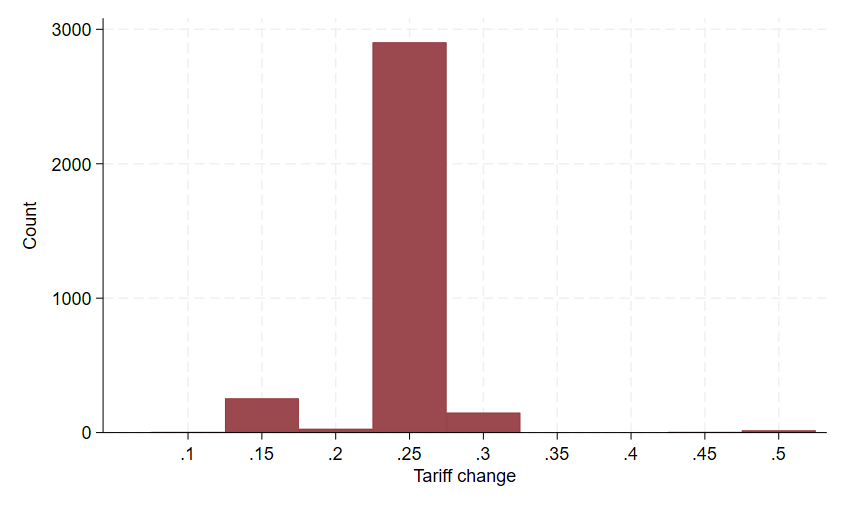
\includegraphics[width=0.85\linewidth]{../Figures/data_figures/tariff_distribution.png}
        \caption{Distribution of tariffs by size in waves 1-3}
        \label{fig:tariff_distribution}
    \end{figure}

    % US ITC tariff data
    \begin{table}[h]
        \centering
        \caption{US ITC tariff data \autocite{amiti_whos_2020}}
        \begin{tabular}{p{3cm} p{2cm} p{2cm} p{2cm} p{2cm} p{2cm}}
            \hline
            \textbf{Variable} & Obs & Mean & Stdev & Min & Max \\
            \hline
            \\[-1.5ex]
            $\textbf{Initial tariff}_{ijt}$ & 23,959,720 & 0.039 & 0.066 & 0 & 3.549 \\[1ex]
            $\textbf{Added tariff}_{ijt}$ & 39,511 & 0.158 & 0.105 & -0.25 & 0.5 \\[1ex]
            $\textbf{Total tariff rate}_{ijt}$ & 23,959,720 & 0.042 & 0.070 & 0 & 3.548 \\[1ex]
            $\textbf{New tariff}_{ijt}$ & 24,449,230 & 0.0016 & 0.0402 & 0 & 1 \\[1ex]
        
        \end{tabular}
    \end{table}

    % Average tariffs - counts: 4, 210, 28, 5, 148, 0,0,4, 16
    \begin{figure}[H]
        \centering
        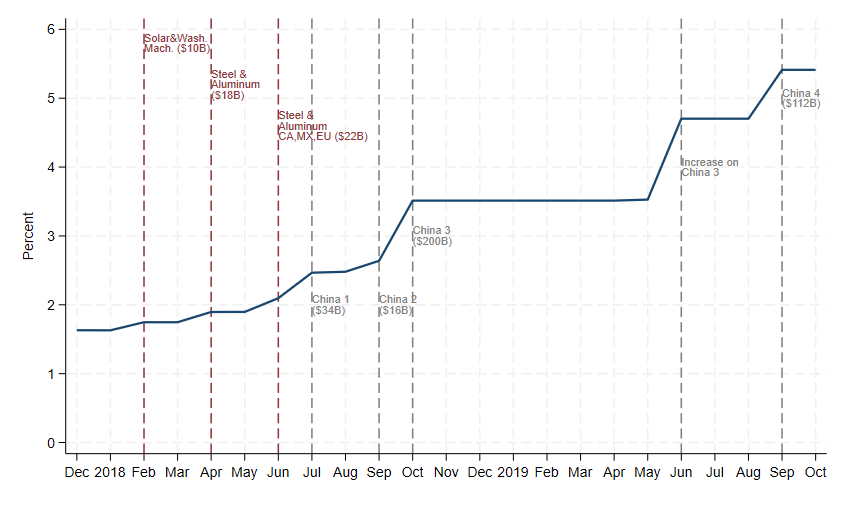
\includegraphics[width=0.85\linewidth]{../Figures/data_figures/average_tariffs.png}
        \caption{Average US tariffs by wave of the 2018-2019 trade war}
        \label{fig:average_tariffs}
        \begin{singlespace}
            \par\noindent\begin{minipage}{0.85\linewidth}
                \footnotesize\textit{Note:} Dashed vertical lines indicate the implementation of each of the eight major waves of new tariffs during the 2018-2019 trade war. This paper studies only the earliest three waves (denoted with maroon lines). Tariffs implemented after the fifteenth of the month counted for the subsequent month. Calculations of average tariffs are based on annual import value across all products in 2017. This graph is sourced from \textcite{amiti_whos_2020}
            \end{minipage}
        \end{singlespace}
    \end{figure}

The United States imposed tariffs relatively consistently in these first three waves, with a modal 25\% tariff applied to nearly 3,000 country and 10-digit product pairs.  

\subsubsection{Trade Agreements}

    % US trade agreements: chart
    \begin{figure}[H]
        \centering
        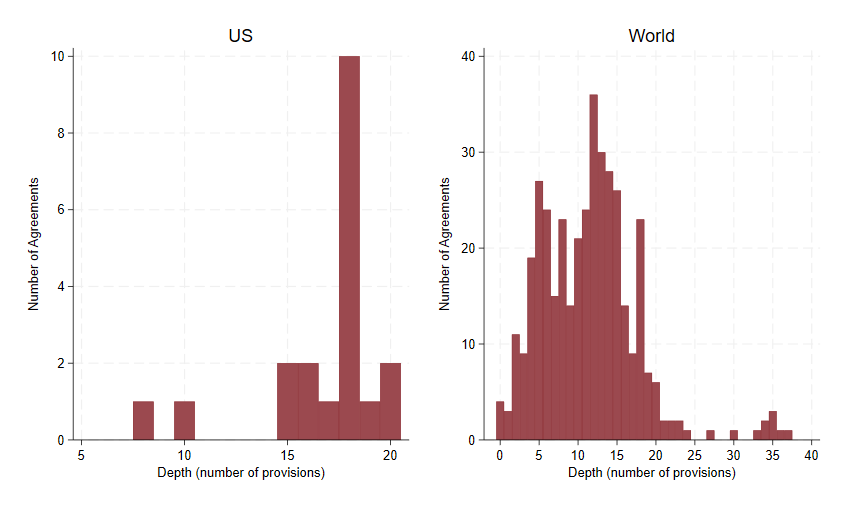
\includegraphics[width=0.85\linewidth]{../Figures/data_figures/us-global_tradeagreements_hist.png}
        \caption{US and Global trade agreements by depth, 2024}
        \label{fig:us-global_trade_agreements_chart}
    \end{figure}

\textcite{mattooTradeCreationTrade2022} define the deepest trade agreements as those with legally enforceable provisions in 20 or more policy areas beyond WTO requirements. Applying this threshold to the US sample would restrict the treated group to NAFTA and USMCA --- effectively, Mexico and Canada alone. Lowering the threshold to 10 legally enforceable provisions, which \textcite{mattooTradeCreationTrade2022} classify as medium-depth, expands the sample to 19 of the 20 countries with which the US has a bilateral trade agreement; only Jordan falls below this cutoff. Any intermediate threshold would be arbitrary, and given the clustering of US agreements between 15 and 20 provisions (Figure~\ref{fig:us-global_trade_agreements_chart}), results would be highly sensitive to the chosen cutoff. I therefore redefine the treatment variable as a binary indicator for whether a country has any bilateral trade agreement with the US, and interpret results accordingly. The original question --- whether deeper trade agreements mitigate tariff shocks --- is examined in robustness checks that vary the depth threshold.

Figure~\ref{fig:us-global_trade_agreements_chart} also shows that the global distribution of trade agreements is substantially shallower than the US distribution. Two implications follow. First, the depth effect could be studied in contexts with greater variation across countries. Second, because US agreements are uniformly deep relative to the global distribution, the resilience effects identified in this paper cannot be extrapolated to trade agreements in general.

\begin{table}[H]
    \centering
    \caption{Sample composition matrix (country-product pairs)}
    \begin{tabular}{l c c c}
        \hline\hline
        & \textbf{Tariffed} & \textbf{Non-tariffed} & \textbf{Total} \\
        \hline
        \textbf{Deep} & 1,280 & 2,387 & 3,667 \\
        & 6.4\% & 11.9\% & 18.3\% \\
        \textbf{Non-deep} & 5,355 & 10,989 & 16,344 \\
        & 26.8\% & 54.9\% & 81.7\% \\
        \hline
        \textbf{Total} & 6,635 & 13,376 & 20,011 \\
        & 33.2\% & 66.8\% & 100\% \\
        \hline\hline
        \multicolumn{4}{l}{\footnotesize\textit{Note:} Count of country-product-month observations = 249,123.}\\
    \end{tabular}
\end{table}

\subsubsection{Trade}

    \begin{figure}[H]
        \centering
        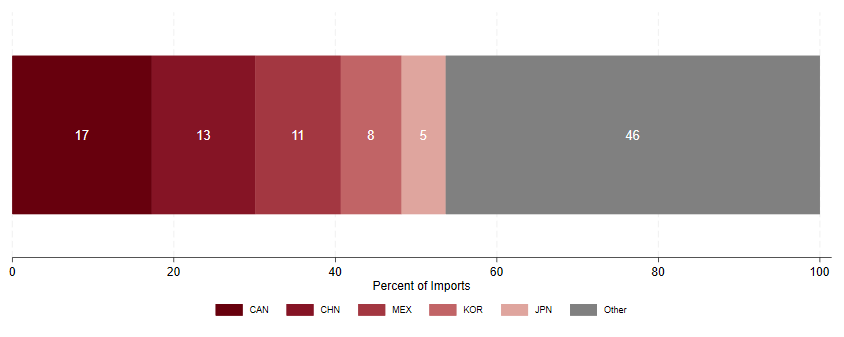
\includegraphics[width=0.75\linewidth]{../Figures/data_figures/total_imports_bycountry_stacked.png}
        \caption{Total US Imports by Source Country, 2017}
        \label{fig:total_imports_bycountry_stacked}
    \end{figure}

    \begin{figure}[H]
        \centering
        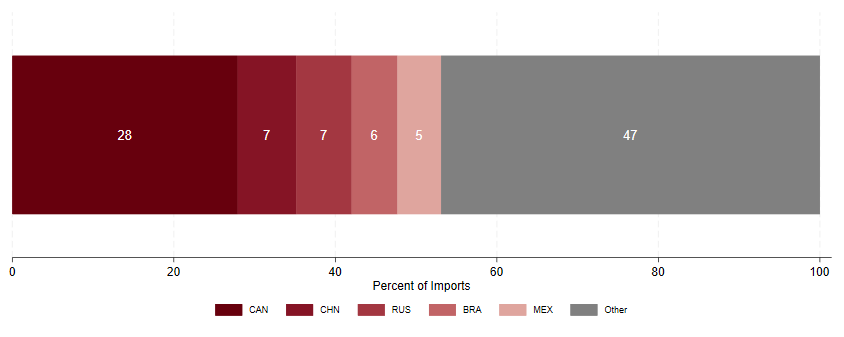
\includegraphics[width=0.75\linewidth]{../Figures/data_figures/steel_imports_bycountry_stacked.png}
        \caption{US Steel Imports by Source Country, 2017}
        \label{fig:steel_imports_bycountry_stacked}
        
        \begin{singlespace}
            \par\noindent\begin{minipage}{0.75\linewidth}
                \footnotesize\textit{Note:} Figures \ref{fig:total_imports_bycountry_stacked} and \ref{fig:steel_imports_bycountry_stacked} are based on the sample of products tariffed in the first three waves at the HS4 level. $N = 249{,}123$ observations at the country-product-month level.
            \end{minipage}
        \end{singlespace}

    \end{figure}

Figures \ref{fig:total_imports_bycountry_stacked} and \ref{fig:steel_imports_bycountry_stacked} show the source composition of US imports in 2017, the pre-tariff baseline year. Across all goods, Canada (17\%), China (13\%), and Mexico (11\%) are the three largest suppliers, with Korea (8\%) and Japan (5\%) rounding out the top five; the remaining 46\% is distributed across 149 other countries. The steel-specific composition differs markedly: Canada accounts for 28\% of steel imports while China supplies only 7\%, consistent with \citeauthor{amiti_whos_2020}'s (\citeyear{amiti_whos_2020}) observation that China is a relatively minor steel supplier to the US market. Russia and Brazil each contribute 7\% and 6\% respectively, with Mexico at 5\%, with the remaining 47\% distributed among 107 other countries. The relative absence of China and relative diversity of suppliers motivates the paper's focus on waves 1–3 of the tariff sequence rather than the China-specific Section 301 waves.

    \section{Models}\label{sec:models}

Following \textcite{amiti_whos_2020}, I estimate the effect of tariffs on prices and volumes using a dynamic event study framework with fixed effects, which has a difference-in-differences interpretation. The outcome variable and the change in tariffs are both logged, permitting the interpretation of the difference-in-differences coefficient as the elasticities of prices and volumes with respect to tariffs. As discussed earlier, I introduce a dummy variable for whether a country does or does not have a trade agreement. This permits a triple-difference interpretation. 

To calibrate the model and understand how this restricted sample compares to the universal results produced by \textcite{amiti_whos_2020}, I initially use the static event study model

    \begin{equation}
        \ln x_{ijt} = \eta_{ij} + \delta_{jt} + \mu_{it} + \sum_{s = -\underline{T}}^{\overline{T}} \beta_s \left( \mathbf{1}_{ijs} \times \ln \left( \frac{1 + \mathit{tariff_{ijs}}}{1 + \mathit{tariff_{ij0}}} \right) \right) \notag + \epsilon_{ijt}
        \label{eq:calibration}
    \end{equation}

where $x$ is the outcome variable, defined as either price or volume, and $\mathbf{1}_{ijs}$ represents a vector of binary indicator variables for each month in $T$, where $-T$ and $T$ are the lower and upper bounds of the event estimation window. The estimation window extends from 12 months before the last untreated month to 12 months after, indicated by $-\underline{T} <= s <= {\overline{T}}$ where $T=24$. The specification uses the log change in tariffs imposed on a country-product pair compared to the last pre-treatment month, where the pre-treatment month $t=0$ is defined as the month before tariffs were applied, and is used as the omitted baseline. The model's coefficients are therefore interpretable as outcome variable's elasticity with respect to log change in tariffs -- the percent difference in prices between a tariffed and non-tariffed product at that particular month. Thus, a country-product pair $ij$ with a 10\% tariff imposed on it will have a price or volume $(\beta_{ijs} \times 100)\%$ higher on average than an untariffed product in the given month $s$. This specification also implies that each coefficient represents the elasticity of the outcome variable with respect to log change in tariffs relative to the omitted baseline -- the last untreated month. 

Following \textcite{amiti_whos_2020}, I include country-product ($\eta_{ij}$), product-time ($\delta_{jt}$), and country-time ($\mu_{it}$) fixed effects. $\eta_{ij}$ absorbs time-invariant factors such as quality or comparative advantage that may influence bilateral trade volumes or prices. $\delta_{jt}$ absorbs time-varying factors that affect US imports of a particular product from all source countries, such as common technological change or changing consumer preferences. Finally, $\mu_{it}$ absorbs time-varying factors that affect imports from a particular country across all products, such as exchange rate fluctuation. To ensure the sample is comparable across tariffed and non-tariffed products, I follow \textcite{amiti_whos_2020} in restricting the sample to HS4 categories affected by at least one of the first three tariff waves. 

I apply this model to the data after restricting the sample to the first three tariff waves. This allows for a comparison of the restricted sample's trends to the general trends observed by Amiti, which can clarify the interpretation of the differential effect of trade agreements on the effect of tariffs, as the restricted sample may not be representative of all country-product combinations. 

% variables in dynamic event study without heterogeneity
\begin{table}[H]
    \centering
    \caption{Model variables and descriptions}\label{tab:model_variables}
    \begin{tabular}{p{0.14\linewidth} p{0.38\linewidth} p{0.38\linewidth}}
        \hline
        \textbf{Variable} & \textbf{Description} & \textbf{Purpose}\\
        \hline
        $\ln x_{ijt}$ & Log import price or value for source country $i$ and product $j$ at time $t$. & This allows the interpretation of the outcome variable as a percent change. \\[1ex]
        $\eta_{ij}$ & Country-product fixed effect. & This absorbs time-invariant factors such as quality or comparative advantage that may influence bilateral trade volumes or prices. \\[1ex]
        $\delta_{jt}$ & Product-time fixed effect. & This absorbs time-varying forces that affect imports of a particular product across all countries (e.g. common technological change). \\[1ex]
        $\mu_{it}$ & Country-time fixed effect. & This absorbs time-varying forces that affect imports from a particular country across all products (e.g. exchange rates). \\[1ex]
        $\mathbf{1}_{ijs}$ & Dummy equal to one when the observation is after a tariff was imposed, where $t=0$ is the last untreated month and the excluded period. & \\[1ex]
        $\ln \left( \frac{1 + tariff_{ijs}}{1 + tariff_{ij0}} \right)$ & Log change in tariffs between month $s$ and the last untreated month $s=0$ for country $i$ and product $j$. & This allows the interpretation of the coefficient $\beta_s$ as the outcome variable's differential elasticity of tariff increases. \\[1ex]
        \hline
    \end{tabular}
\end{table}

I then run the following regression, separating it by bilateral trade agreement status

    \begin{equation}
        \begin{gathered}
            \ln x_{ijt} = \eta_{ij} + \delta_{jt} + \mu_{it} + \sum_{s = -\underline{T}}^{\overline{T}} \beta_s^{A} \left( \mathbf{1}_{ijs} \times \ln \frac{1 + \mathit{tariff}_{ijs}}{1 + \mathit{tariff}_{ij0}} \right) + \varepsilon_{ijt}, \\
            A \in \{\textnormal{agreement}, \textnormal{no agreement}\}
        \end{gathered}
        \label{eq:agreement}
    \end{equation}

where $A$ indicates whether the regression is run on the subsample of countries with trade agreements or without trade agreements. This is once again a dynamic event study framework using fixed effects with a difference-in-differences interpretation, where the first difference is between pre and post-treatment, and the second difference is between tariffed and non-tariffed country-product pairs. This specification results in two regressions: one for each subsample by bilateral trade agreement status. I then compute the difference between the corresponding coefficients across the two regressions using the difference in means that also combines the coefficients' confidence intervals. This results in a triple-differences interpretation, where the first difference is between pre and post-treatment, the second difference is between tariffed and non-tariffed country-product pairs, and the third difference is between countries with and without bilateral trade agreements with the US. 

To investigate further heterogeneities, I run the following regression -- essentially Equation~\ref{eq:heterogeneity} applied to each subgroup of interest: 

    \begin{equation}
        \begin{gathered}
            \ln x_{ijt} = \eta_{ij} + \delta_{jt} + \mu_{it} + \sum_{s = -\underline{T}}^{\overline{T}} \beta_s^{A,B} \left( \mathbf{1}_{ijs} \times \ln \frac{1 + \mathit{tariff}_{ijs}}{1 + \mathit{tariff}_{ij0}} \right) + \varepsilon_{ijt}, \\
            A \in \{\textnormal{agreement}, \textnormal{no agreement}\}
        \end{gathered}
        \label{eq:heterogeneity}
    \end{equation}

where $B$ is the group of interest. 

% ---------------------------------------------------------------%
% ---------------------------------------------------------------%
  
    \section{Results}\label{sec:results}
The specification uses a triple-difference interpretation. The three differences are: (i) between pre- and post-treatment periods, (ii) between tariffed and non-tariffed products, and (iii) between deep and non-deep trade agreement countries. This design allows me to examine whether trade agreement depth moderates the effect of tariffs on import prices. As formalized by \textcite{oldenTripleDifferenceEstimator2022}, valid triple-difference interpretation requires that the relative performance of tariffed versus non-tariffed products be similar across deep and non-deep countries prior to treatment. This assumption is addressed throughout this section. 

\subsection{Sample calibration}

    \begin{figure}[h]
        \centering
        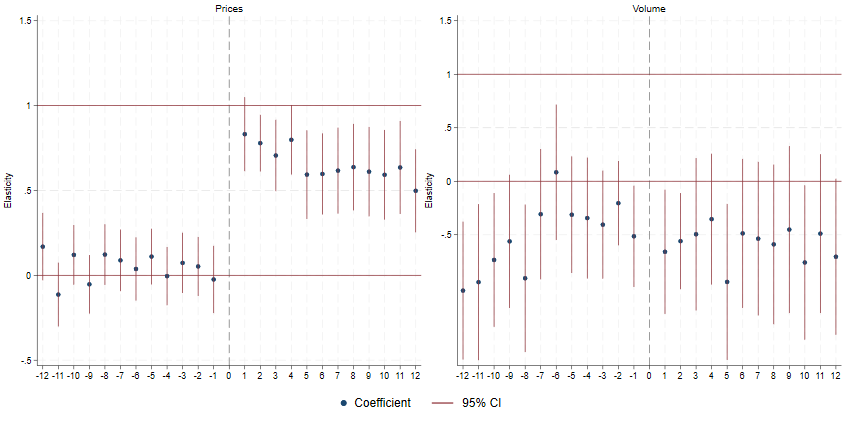
\includegraphics[width=0.85\linewidth]{../Figures/reg_figures/reg_baseline_combined.png}
        \caption{Sample calibration regression results}
        \label{fig:sample_calibration}
    \end{figure}

As seen in Figure~\ref{fig:sample_calibration}, the restricted sample's prices behave similarly to the complete pass-through found in \textcite{amiti_whos_2020}. In contrast to the universal sample's sustained and steady complete pass-through, it appears that within this sample, pass-through approached one initially before declining to approximately 0.5. This is most consistent with Amiti's findings for steel inputs, which show steel prices to follow a nearly identical pattern with minor variations. Pre-trends, meanwhile, are statistically indistinguishable from zero, indicating zero pre-trends are likely. This was also the case in Amiti's sample --- both universal and specific to steel. 

Volumes exhibit some pre-trends, with volume elasticity rising slightly before stabilizing over -0.5 at 6 months before treatment. Following treatment, we see no meaningful change, but for a slight increase in the four months after tariff implementation and a subsequent noisy decline. Overall, confidence intervals are wide and steadily occupy roughly the same area, between approximately 0 and -1. The results in \textcite{amiti_whos_2020} exhibit a small negative but rising volume elasticity between 12 and 6 months prior to treatment, before steadily declining across the board following tariff implementation. Steel products experienced the smallest negative elasticity, never reaching far below -1. This roughly matches the restricted sample, though the sample's post-treatment outcomes are less clearly identified. 

This sample suggests that tariffs saw incomplete pass-through of tariffs to prices, with a minimal effect on volumes. Of the categories and product types examined in \textcite{amiti_whos_2020}, these trends most closely resemble those of the steel category studied in \textcite{amiti_whos_2020}.\footnote{These charts are available in \autocite{amiti_whos_2020}.}  

\subsection{Differential agreement effect}

    \begin{figure}[H]
        \centering
        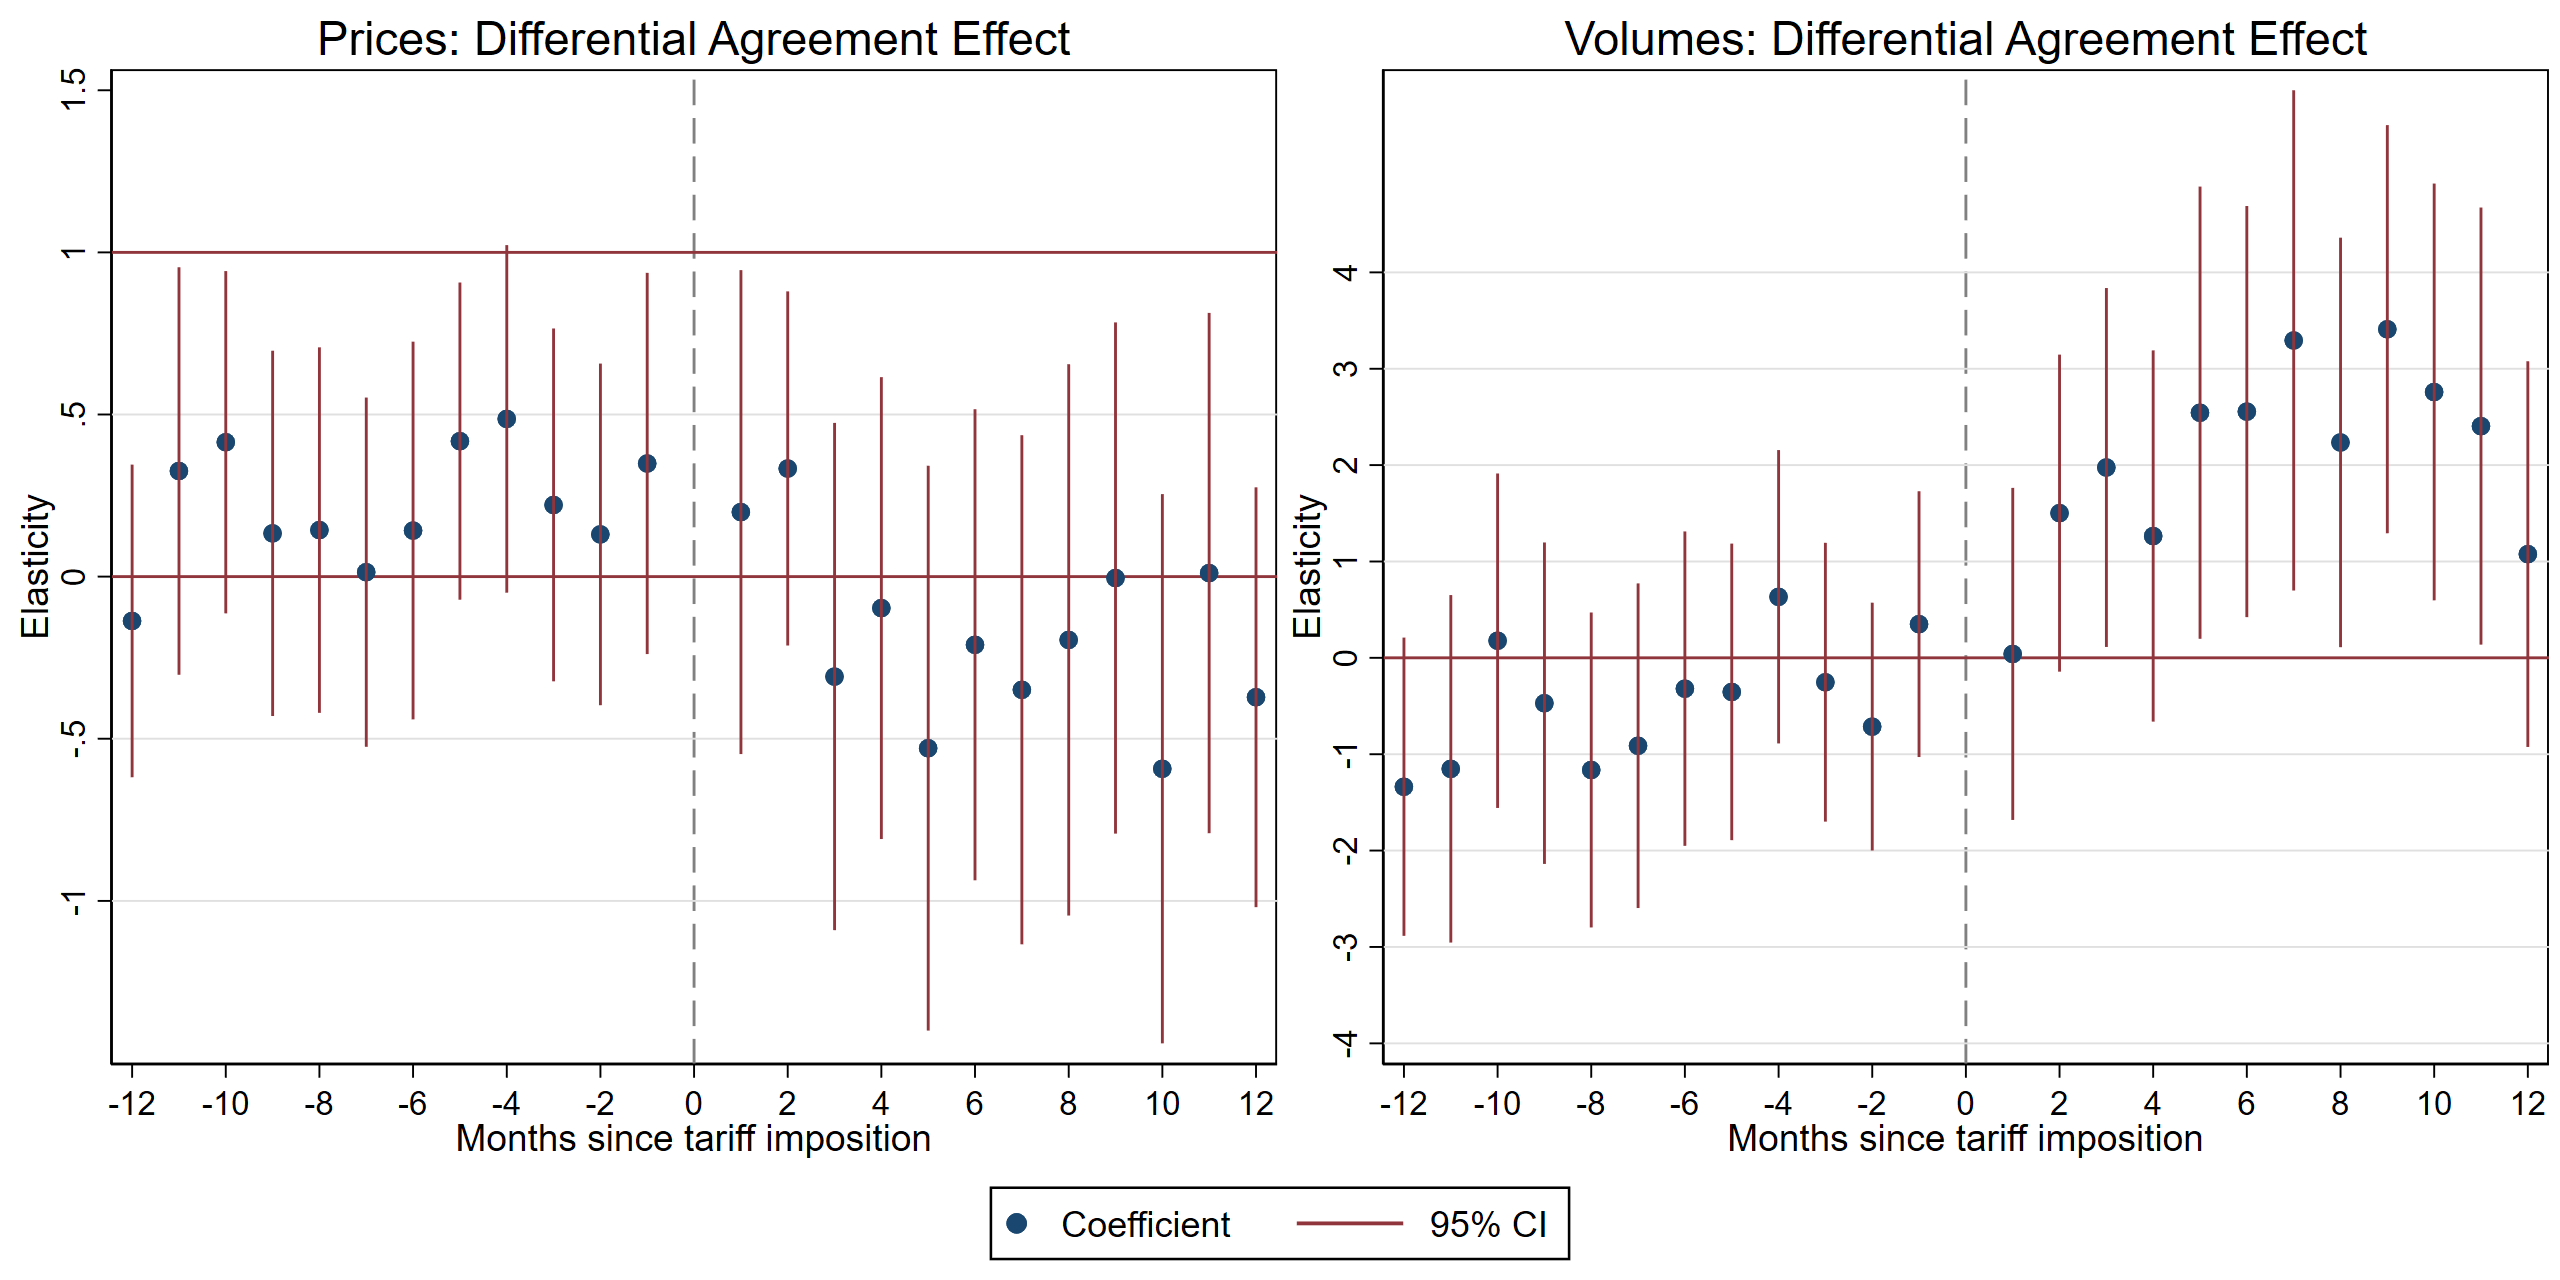
\includegraphics[width=0.85\linewidth]{../Figures/reg_figures/reg_all_diff_combined.png}
        \caption{Agreement vs No agreement regression differences}
        \label{fig:reg_all_diff_combined}
    \end{figure}

The differential effect of trade agreements on prices and volumes is identified by computing the difference between the coefficients for the subsample of countries with bilateral trade agreements and those for the subsample of countries without bilateral trade agreements with the US. These differential outcomes exhibit markedly different patterns than the above regression. The panels in Figure~\ref{fig:reg_all_diff_combined} show the estimated differential monthly elasticities of tariff-inclusive import prices and import volumes for 12 months before and after treatment. While a null effect of trade agreements would require the monthly coefficients to equal zero in both panels, this is evidently not the case.

On the surface, the results suggest that agreement countries experienced smaller price pass-through and a relative increase in import volumes compared to non-agreement countries. Because these coefficients reflect differential effects between the two groups rather than absolute responses, further analysis is required to interpret what they reveal about the effect of tariffs on prices and volumes. Nonetheless, the patterns are consistent with the initial hypothesis that trade flows between the US and its agreement partners would prove more resilient to unilateral tariff shocks.

The differential effect of tariffs on prices for countries with versus without bilateral trade agreements with the US is shown in Figure~\ref{fig:reg_all_diff_combined}. Pre-treatment differential coefficients are consistently positive, though mostly small in magnitude, and statistically indistinguishable from zero in most months, satisfying the parallel trends assumption. Following tariff implementation, the differential remains positive for two months --- in line with pre-treatment coefficients --- before turning negative, where it remains through the rest of the post-treatment window. On the surface, this pattern suggests a delayed moderating effect of trade agreements on tariff pass-through.

The underlying agreement-status regressions in Figure~\ref{fig:reg_all_agrstatus_combined} clarify what is driving this differential. Panel (1) shows that agreement countries experienced a sharp price increase in the first two months following tariff implementation --- larger than the corresponding response in non-agreement countries (panel (2)) --- before settling to a price elasticity slightly below the non-agreement group in subsequent months. What appeared on the surface to be a delayed moderating effect was in fact elevated initial pass-through followed by partial absorption. Although the data is noisy, the consistently negative differential in the medium term indicates that trade agreements have a slightly moderating effect on tariff pass-through to border prices. Section~\ref{sec:interpretation} discusses possible mechanisms.

    \begin{figure}
        \centering
        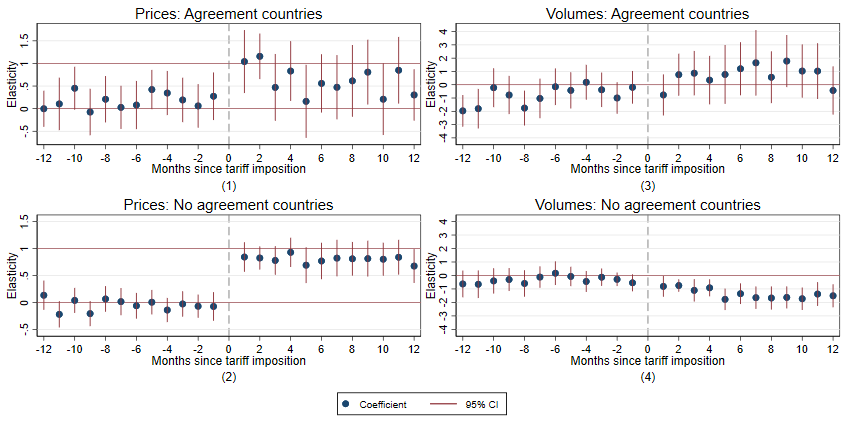
\includegraphics[width=0.85\linewidth]{../Figures/reg_figures/reg_all_agrstatus_combined.png}
        \caption{Agreement vs No agreement regression results}
        \label{fig:reg_all_agrstatus_combined}
    \end{figure}
    
The differential effect of tariffs on volumes (Figure~\ref{fig:reg_all_diff_combined}) exhibits a starker and clearer pattern. Pre-treatment coefficients are statistically insignificant at the 5\% level, indicating no evidence of relative pre-trends. Following tariff implementation, import volumes from agreement countries display substantially higher differential elasticities than non-agreement countries while increasing over time, with the differential ranging from 1 to 3 in most months. Taken at face value, the modal 25\% tariff would --- all else equal --- generate a peak 75\% difference in the volume response between the two groups around eight months after implementation, though wide confidence intervals caution against literal extrapolation. This pattern admits two interpretations: agreement countries may be experiencing a smaller drop in volumes, or an outright rise in volumes while non-agreement countries decline.

Figure~\ref{fig:reg_all_agrstatus_combined} supports the latter. Volumes from agreement countries rise over time (panel (3)), while non-agreement countries' volumes decline steadily for six months following tariff implementation before plateauing at an elasticity slightly above $-2$ (panel (4)). This implies that a 25\% tariff would generate an approximately 44\% decline in imports from non-agreement countries twelve months after implementation, while producing an approximately 25\% rise in imports from agreement countries.

Taken together, the aggregate results indicate that bilateral trade agreements with the US moderate the effects of tariffs on both  prices and volumes, with the volume response substantially clearer than the price response. Agreement countries experience higher initial pass-through that gradually transitions to partial absorption, while their import volumes rise even as non-agreement countries see import volumes fall. These patterns are consistent with the hypothesis that institutionalized trade relationships provide some resilience to unilateral tariff shocks. However, the aggregate sample combines steel and non-steel products, and the close resemblance of these results to the steel-only patterns reported in \autocite{amiti_whos_2020} raises the possibility that steel products, which constitute the majority of the sample, are driving the aggregate findings. Section~\ref{sec:steel_heterogeneity_results} examines whether the differential agreement effect holds within each product category separately.

\subsection{Triple-difference by steel and non-steel products}\label{sec:steel_heterogeneity_results}

\begin{table}[H]
\centering
\caption{Sample decomposition (count of country-product pair)}\label{tab:steel_share}
    \begin{tabular}{c | cc | c}
    \hline
    & \textbf{Steel} & \textbf{Non-steel} & \textbf{Total} \\
    \hline 
                \textbf{Agreement} & 35,130 & 16,262 & 51,392 \\
                & 14.1\% & 6.5\% & 20.6\% \\

                \textbf{No agreement} & 126,196 & 72,535 & 197,731 \\
                & 50.7\% & 29.1\% & 79.8\% \\
            \hline
                \textbf{Total} & 161,326 & 87,897 & 249,123 \\
                & 64.8\% & 35.3\% & 100\% \\        
    \end{tabular}
\end{table}

Table~\ref{tab:steel_share} decomposes the sample by steel and non-steel products, revealing that steel products constitute nearly 65\% of the country-product pairs and 68\% of the agreement subsample.\footnote{Calculation: $14.1\% / 20.6\% = 68.4\%$.} This composition raises two related concerns. First, the close resemblance of the aggregate results to the steel-only patterns reported in \autocite{amiti_whos_2020} could simply reflect that steel observations dominate the aggregate by construction. Second, and more substantively, the differential agreement effect may operate differently across product categories, and the aggregate result could mask meaningful heterogeneity. To distinguish these possibilities, I implement Equation~\ref{eq:heterogeneity} with $B \in \{\textnormal{steel}, \textnormal{non-steel}\}$, estimating the differential agreement effect separately within each product category.

\subsubsection{Prices of steel vs. non-steel products}

    % Steel vs non-steel Prices: Differences
    \begin{figure}[H]
        \centering
        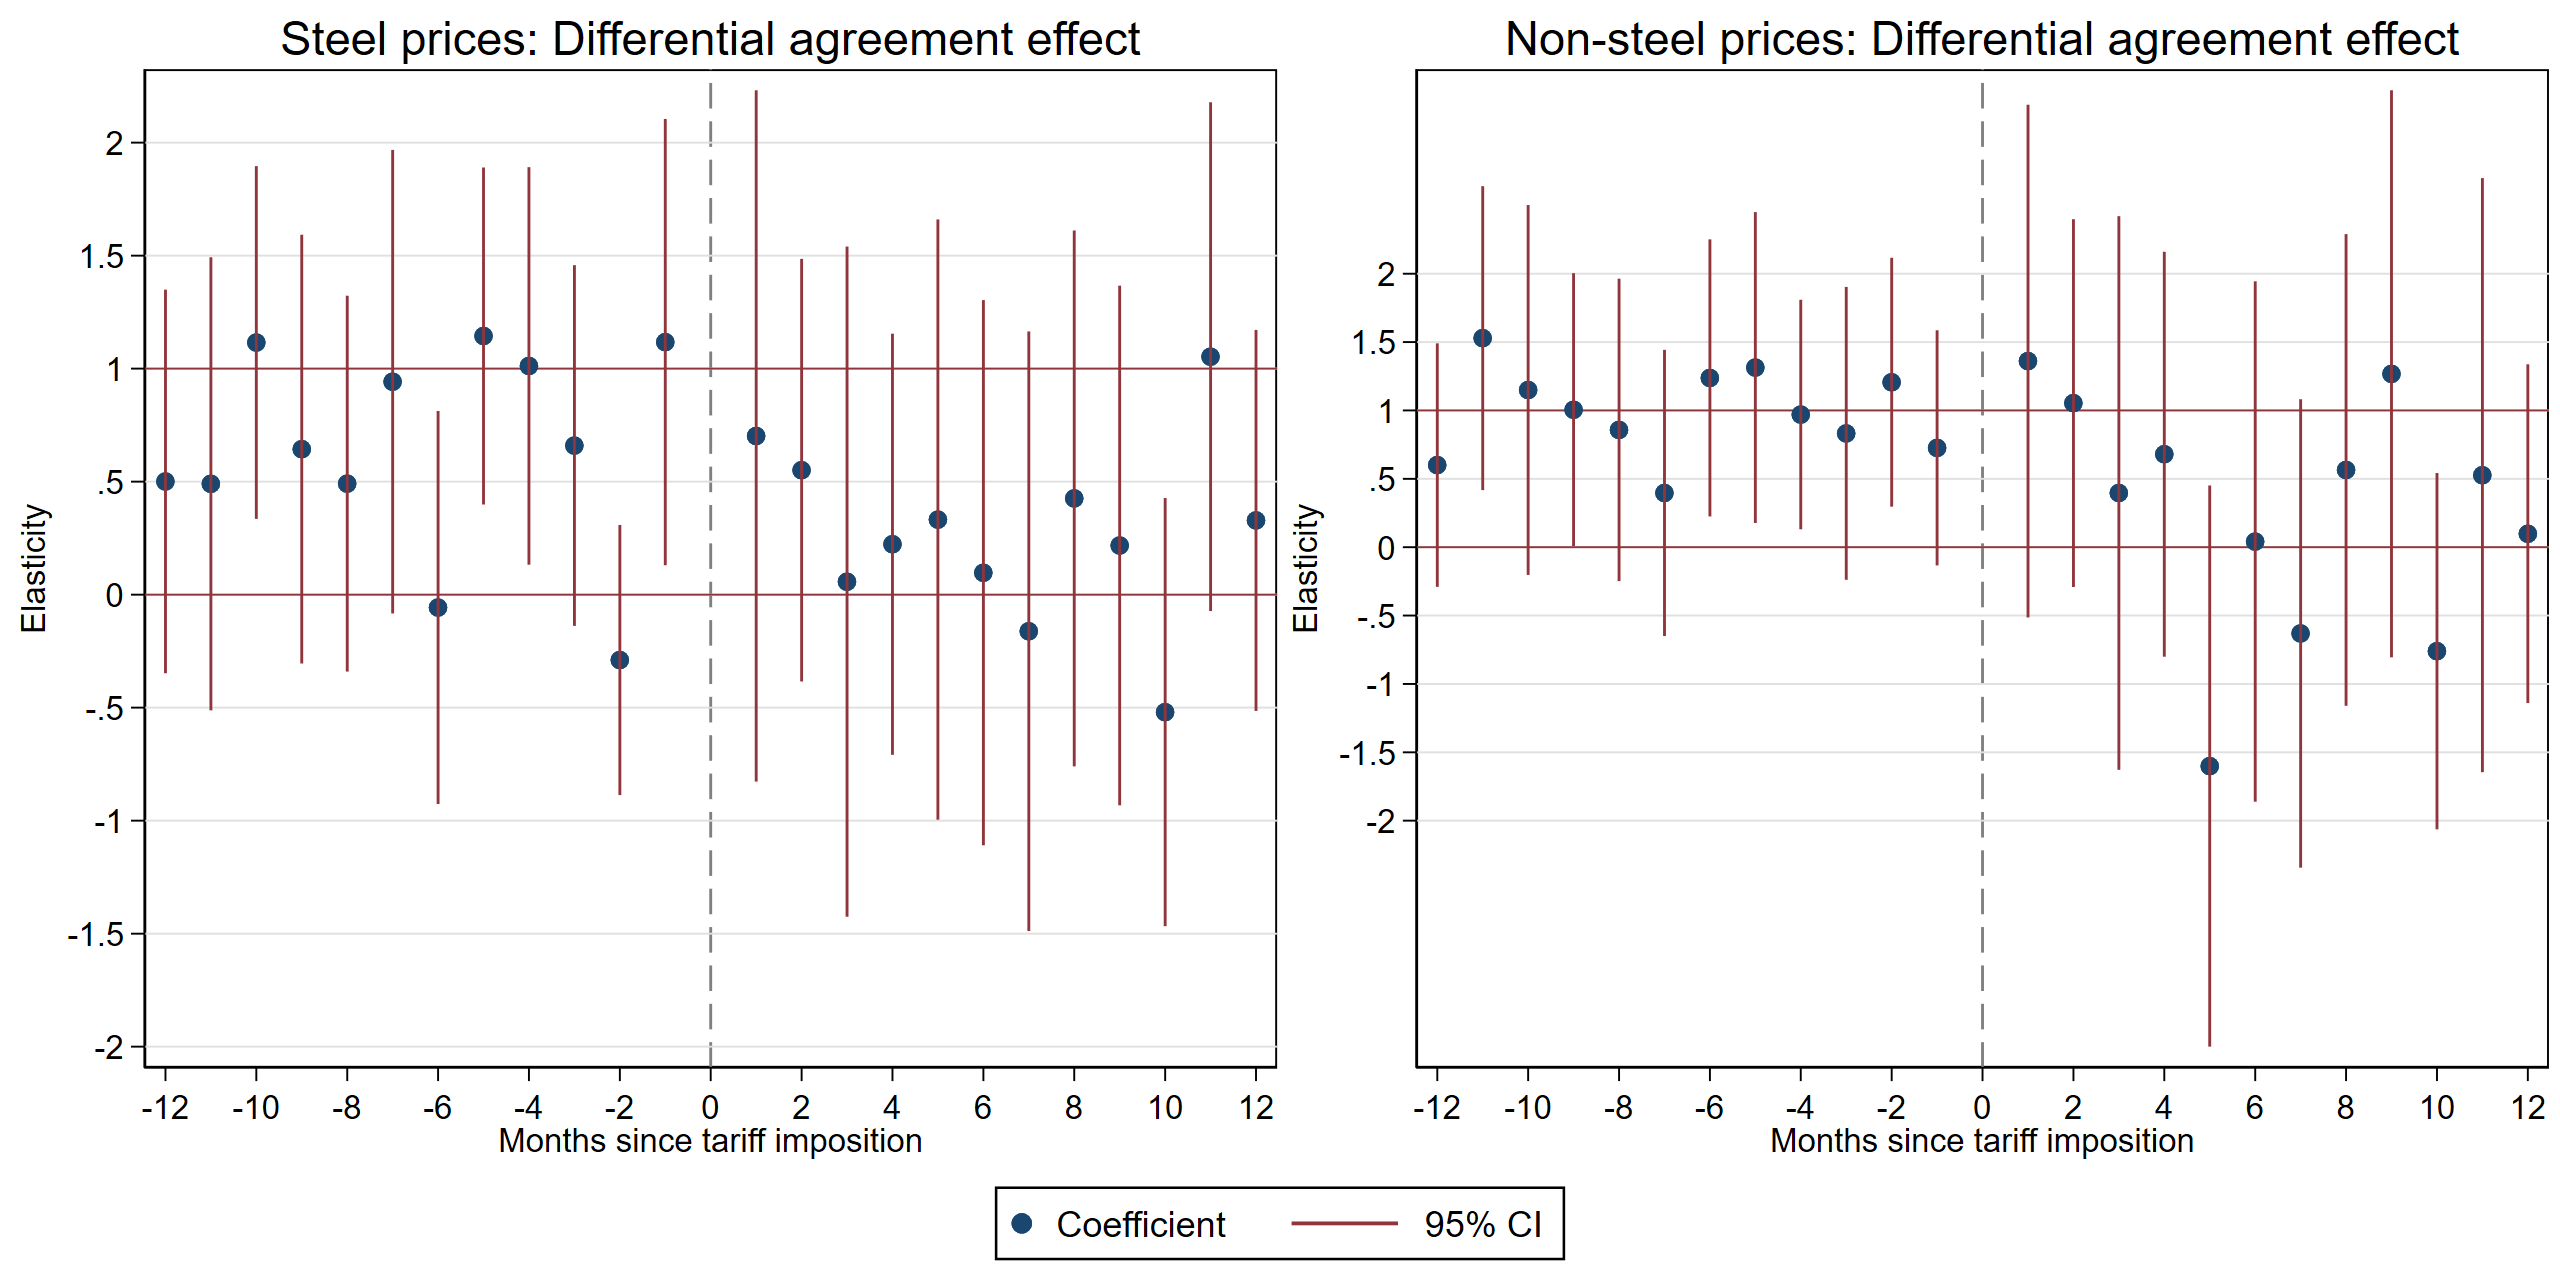
\includegraphics[width=0.85\linewidth]{../Figures/reg_figures/steel_prices_diff.png}
        \caption{Steel vs non-steel prices: Differential effect of agreements}
        \label{fig:steel_prices_diff}
    \end{figure}

    % Steel vs non-steel Prices: By agreement status
    \begin{figure}[H]
        \centering
        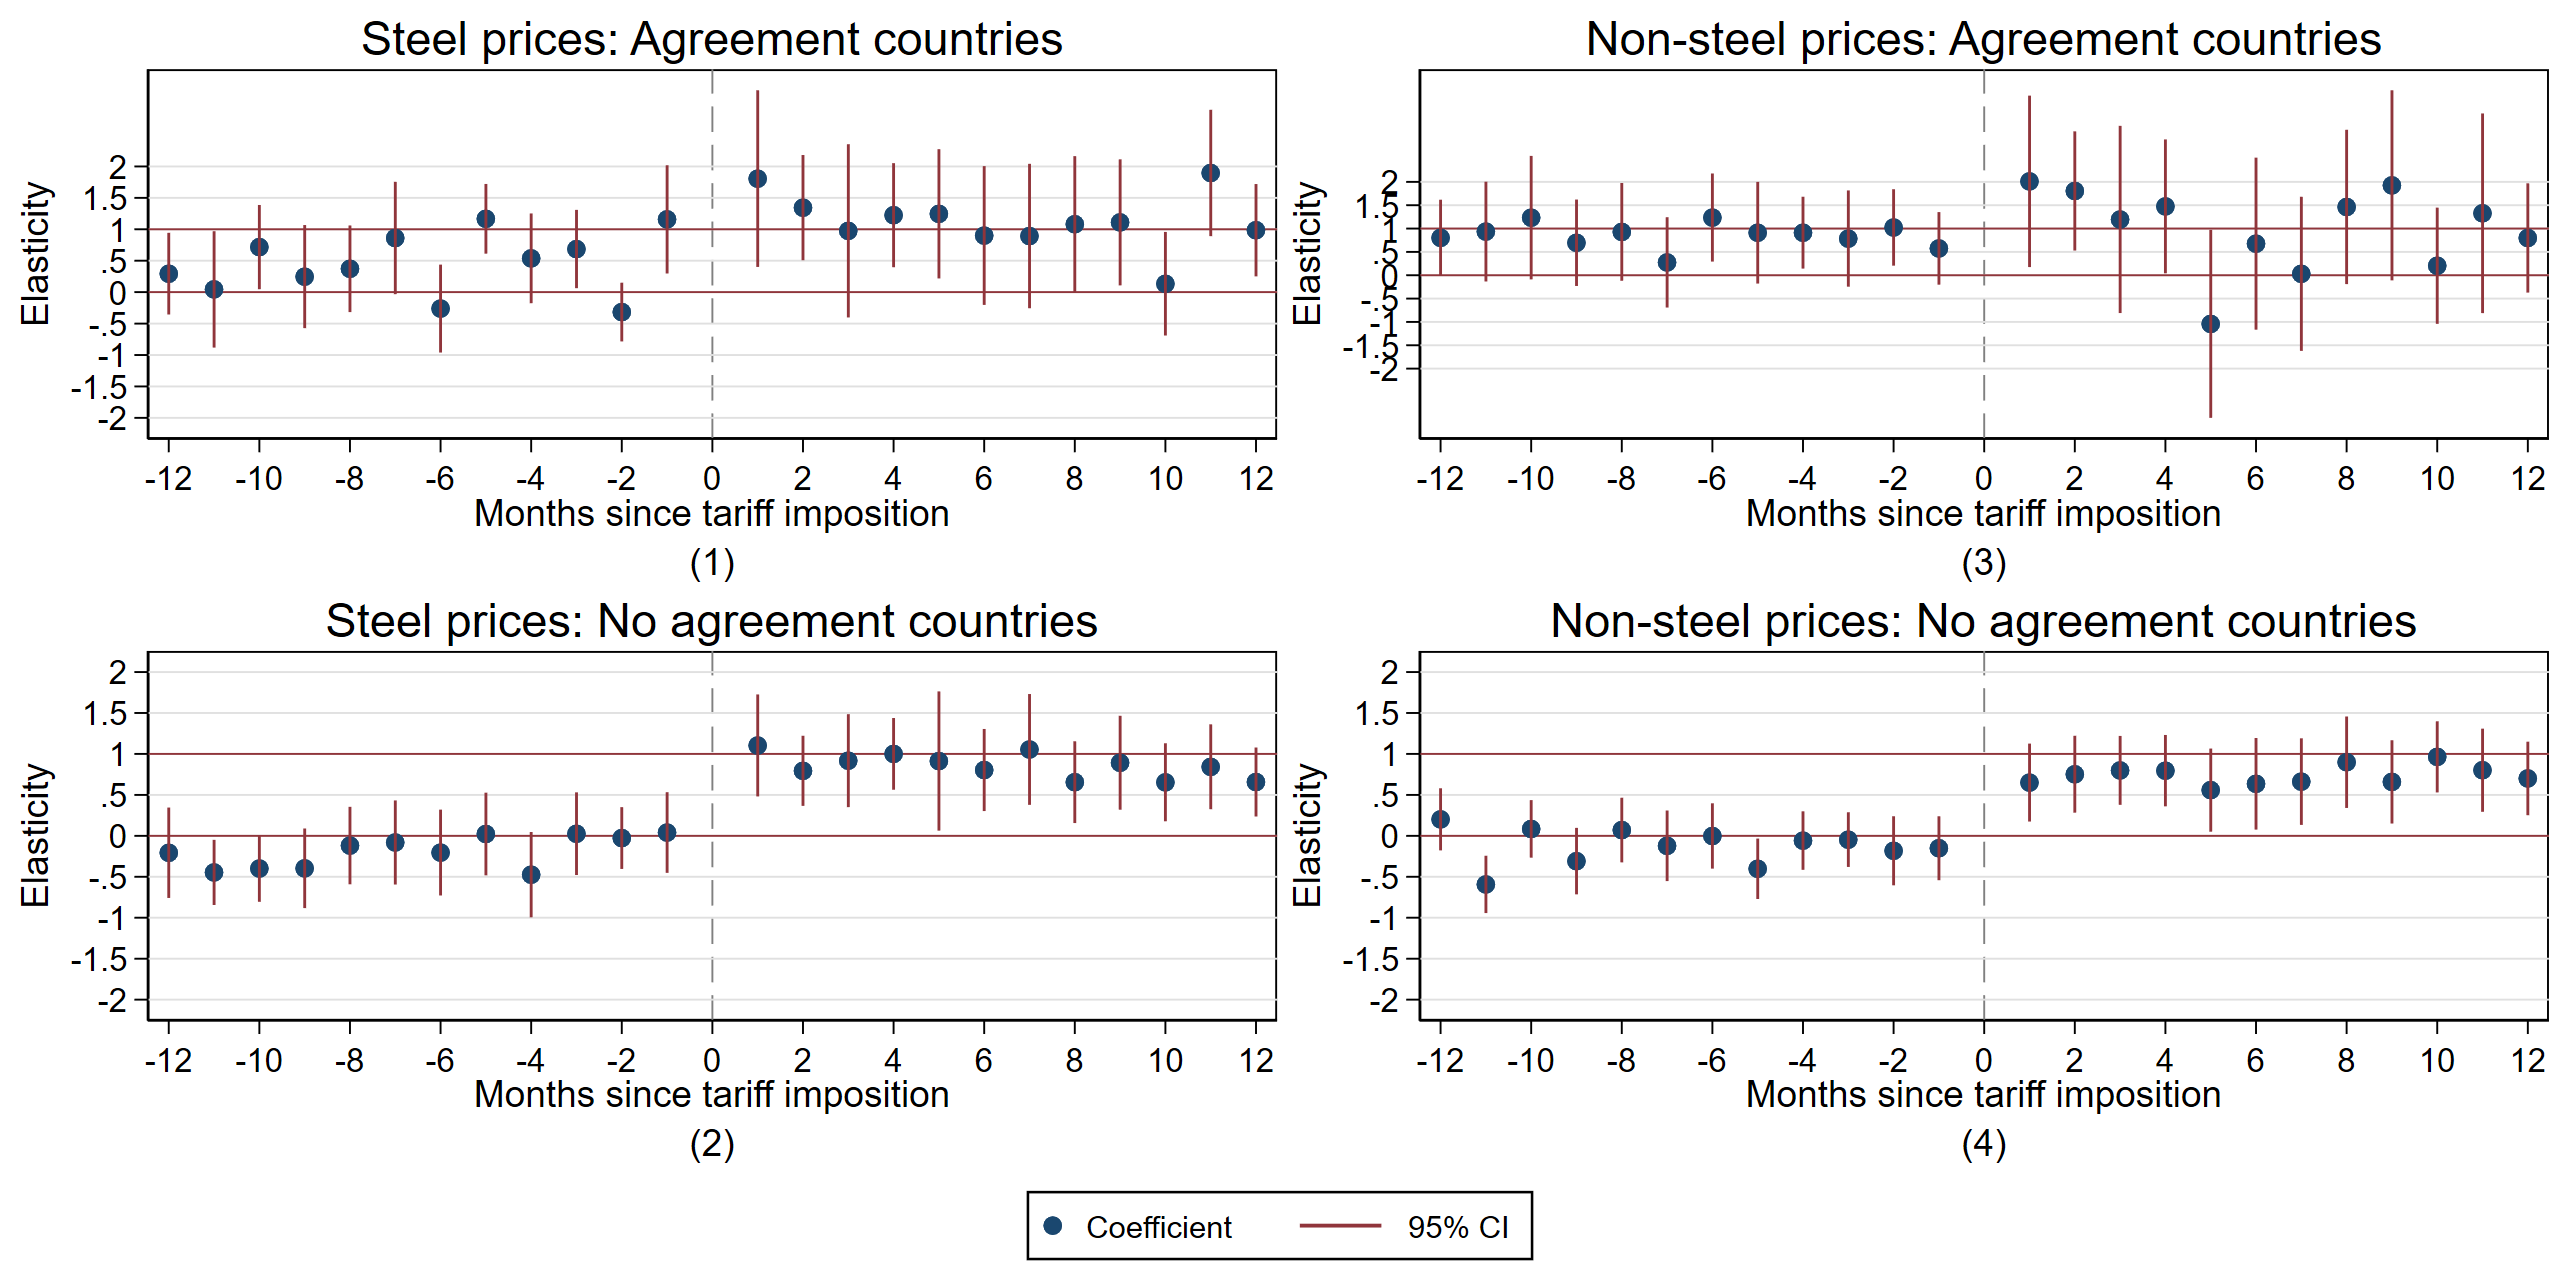
\includegraphics[width=0.85\linewidth]{../Figures/reg_figures/steel_prices_agrstatus.png}
        \caption{Steel vs non-steel prices: Regressions by agreement status}
        \label{fig:steel_prices_agrstatus}
    \end{figure}

Two comparisons help assess whether steel observations dominate the aggregate result. First, comparing the aggregate differential effect (Figure~\ref{fig:reg_all_diff_combined}) to the steel and non-steel differentials (Figure~\ref{fig:steel_prices_diff}) reveals some post-treatment similarity between the aggregate and steel patterns, but substantial differences elsewhere. Both subsample differentials exhibit noisy pre-treatment coefficients with seemingly positive pre-treatment price elasticities, in contrast to the cleaner, nearly null pre-trends in the aggregate. The post-treatment patterns also diverge: while the aggregate differential settles into a consistently negative band, the steel and non-steel differentials are more volatile and less precise. Second, comparing the agreement and non-agreement split-sample regressions across the aggregate (Figure~\ref{fig:reg_all_agrstatus_combined}) and the product-category subsamples (Figure~\ref{fig:steel_prices_agrstatus}) shows that within each agreement-status group, the steel and non-steel coefficients appear statistically indistinguishable based on overlapping confidence intervals. 

Together, these comparisons suggest that the differential agreement effect is not mechanically driven by the steel-heavy composition of the aggregate sample. Although steel observations constitute the majority of the data, the steel and non-steel subsamples do not exhibit meaningfully different differential agreement effects, and the aggregate result appears to reflect a pattern that holds across both product categories rather than one driven by steel alone. The pre-trend concerns raised by the subsample comparisons, however, warrant closer examination, which the following analysis addresses.

Figures~\ref{fig:steel_prices_agrstatus} and \ref{fig:steel_prices_diff} reveal a pre-trend violation that undermines causal interpretation of the agreement differential with respect to prices. Within both steel (Fig. \ref{fig:steel_prices_agrstatus} (1)) and non-steel (Fig. \ref{fig:steel_prices_agrstatus} (3)) products, agreement countries exhibit systematically positive pre-treatment price coefficients while non-agreement countries display null pre-trends (Fig. \ref{fig:steel_prices_agrstatus} (1) and (3)), generating a positive agreement/non-agreement differential prior to tariff implementation. Since all coefficients are defined relative to the last pre-treatment month, these positive pre-period coefficients imply the differential was elevated in earlier months and declined into the baseline, before recovering post-treatment. This pattern is inconsistent with the parallel trends assumption required for causal identification of price elasticity in this context: the differential was already moving before tariffs were imposed, and post-treatment estimates cannot be cleanly attributed to tariff pass-through heterogeneity by whether or not countries have trade agreements with the United States. One source of this instability could be heterogeneity between steel products sourced from countries with versus  without trading agreements, coupled with a smaller set of countries within the agreement subsample. Steel and non-steel products from countries with US trade agreements may fundamentally be different from global products, resulting in some pre-trends. As a result, the product-time fixed effect $\delta_{jt}$ may be absorbing fundamentally different variation that explains the discrepancy. Another could be that perhaps the pre-treatment month is anomalous in some way, perhaps due to anticipation of tariffs. 

Accounting for the fact that there may be some distortion in the pre-treatment sample, it does appear that for both steel and non-steel products, there is some effect of tariffs within imports from countries with trade agreements. Elasticity for steel products from this group of countries (Fig. \ref{fig:steel_prices_agrstatus} (1)) fluctuates between 0 and 1 before tariff implementation, but rises afterwards. Once tariffs are imposed, elasticity jumps to about 2 before declining to a tight band around 1. In any case, there is a clear difference --- taking the approximately 0.5 elasticity pre-treatment coefficients hover around at face value, it seems there is an increase in pass-through due to tariffs within this group to the magnitude of approximately 0.5 relative to the pre-treatment elasticity. Comparing this directly to the effect of tariffs on steel prices within the non-agreement group, it appears that agreement countries experienced a slightly smaller increase in price elasticities following tariffs' imposition. Based on this comparison of pre- and post-treatment elasticities, it appears that in fact, countries with trade agreements did indeed have lower pass-through than agreement countries. This cannot be interpreted causally, however, due to the major violation of the zero relative pre-trends assumption. 

This pattern is replicated in non-steel products. While pre-treatment elasticities are elevated around 1 for agreement countries, they rise to 2 immediately after tariffs are imposed before declining over the first quarter. Following this, elasticities fluctuate dramatically. While this is likely a result of the small sample size for non-steel country-product pairs where the country has a trade agreement with the US (N=16,262), the difference between the pre-treatment and post-treatment elasticities for agreement countries appears once again to be slightly smaller on average than for non-agreement countries. Meanwhile, this volatility is notable, particularly as the coefficients remained in a relatively narrow band before implementation. This fluctuation suggests there could be a high degree of heterogeneity within this subsample in how foreign exporters respond to tariffs. 

\subsubsection{Volume of steel vs. non-steel products}

    % Steel vs non-steel Volume: Differences
    \begin{figure}[H]
        \centering
        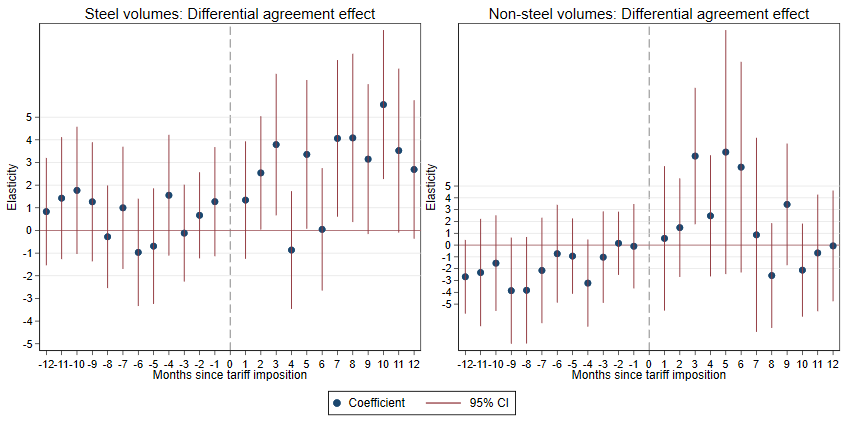
\includegraphics[width=0.85\linewidth]{../Figures/reg_figures/steel_volume_diff.png}
        \caption{Steel vs non-steel volumes: Differential effect of agreements}
        \label{fig:steel_volume_diff}
    \end{figure}

    % Steel vs non-steel Volume: By agreement status
    \begin{figure}[H]
        \centering
        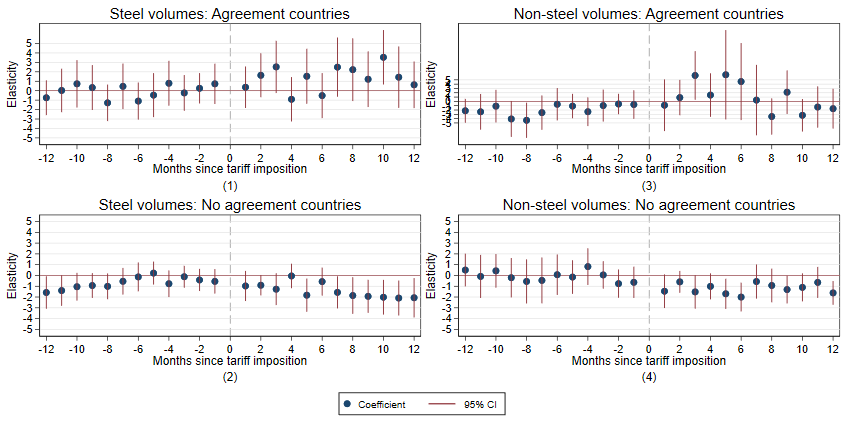
\includegraphics[width=0.85\linewidth]{../Figures/reg_figures/steel_volume_agrstatus.png}
        \caption{Steel vs non-steel volumes: Regressions by agreement status}
        \label{fig:steel_volume_agrstatus}
    \end{figure}

To assess whether the differential effect of agreements on volume elasticities is driven by the dominant steel subsample, I repeat the same exercise as above. First, comparing the aggregate differential (Figure~\ref{fig:reg_all_diff_combined}) to the steel and non-steel differentials (Figure~\ref{fig:steel_volume_diff}), the steel differential closely resembles the aggregate, while the non-steel differential is broadly similar in the first six post-treatment months before diverging substantially after seven months. Second, examining the agreement and non-agreement split samples within each product category (Figure~\ref{fig:steel_volume_agrstatus}) reveals that within the non-agreement group, steel and non-steel exhibit similar volume elasticities and both resemble the aggregate non-agreement pattern. Within the agreement group, however, the steel and aggregate patterns align, while the non-steel pattern diverges after seven months post-tariff implementation, dropping into negative elasticity territory.

This decomposition suggests that the steel subsample does drive the aggregate agreement-country result. The aggregate increase in volume elasticities observed for agreement countries reflects the steel-specific pattern, while non-steel agreement-country volume elasticities follow an initially positive trajectory before turning negative. The non-agreement results, by contrast, are consistent across product categories and are not subject to this concern. The divergence between steel and non-steel within the agreement group warrants closer examination, which the following analysis addresses.

Turning to the identification of a differential agreement effect on volume elasticities, the coefficients exhibit clean pre-treatment behavior, in contrast to the ambiguous pre-trends in the price specification. Figure~\ref{fig:steel_volume_diff} shows that the differential volume elasticity is statistically indistinguishable from zero in the pre-treatment period for both steel and non-steel products, satisfying the parallel trends requirement for causal identification of $\beta_s$. Within steel products, agreement countries display a null pre-trend, while non-agreement countries show a slight positive movement between 12 and 6 months prior to treatment (Fig.~\ref{fig:steel_volume_agrstatus}, panels (1) and (2)); this minor deviation does not translate into a meaningful differential, which remains null throughout the pre-period. Within non-steel products, the differential exhibits a slight upward drift, driven by a small positive pre-trend in agreement countries and a small negative pre-trend in non-agreement countries (Fig.~\ref{fig:steel_volume_agrstatus}, panels (3) and (4)). Both group-specific pre-trends remain statistically insignificant in nearly all pre-treatment months, and the differential itself is statistically indistinguishable from zero across both groups. Taken together, the volume specification provides a substantially stronger basis for causal interpretation than the price specification.

Following tariff implementation, the differential volume elasticity is positive for both steel and non-steel products, indicating that agreement countries captured import volume relative to non-agreement countries (Fig.~\ref{fig:steel_volume_diff}). Within steel products, this differential is driven by a large and slightly increasing positive volume elasticity in agreement countries, paired with a negative elasticity in non-agreement countries that fluctuates around $-1$ in the first few post-tariff months before declining further to roughly $-2$ (Fig.~\ref{fig:steel_volume_agrstatus}, panels (1) and (2)). Within non-steel products, the differential is highly positive in the first six months before declining, though all but one month is statistically insignificant (Fig.~\ref{fig:steel_volume_diff}). The agreement-country volume elasticity peaks at approximately 6 around five months post-treatment --- a magnitude that, taken at face value, would imply a $25\%$ tariff generates a $150\%$ increase in import volumes, though the wide confidence intervals at this time horizon caution against literal interpretation. The elasticity subsequently declines, crossing into negative territory after seven months with one outlier, though most post-treatment estimates remain statistically insignificant. By contrast, non-agreement countries exhibit consistently negative non-steel volume elasticities, ranging between $-0.5$ and $-2$ with an average near $-1$, and these estimates are statistically significant in most periods (Fig.~\ref{fig:steel_volume_agrstatus}, panels (3) and (4)).

Taken together, these two exercises reveal that while the subsample is cleanly interpretable with parallel trends satisfied across both product categories, it is not well-balanced. The differential agreement effect on volumes is positive following tariff implementation, indicating that agreement countries captured import share as non-agreement countries lost it. However, this aggregate finding masks heterogeneity: steel products from agreement countries exhibit a large and persistent volume increase, while non-steel products from agreement countries reveal a transient gain that reverses after around six months. Meanwhile, both product categories exhibit consistent volume declines for non-agreement countries. The persistence of the steel trend and the reversal of the non-steel trend suggest that the resilience conferred by trade agreements is product-specific. Coupled with the fact that the first exercise indicates the aggregate sample is dominated by the steel subsample, the model's aggregate findings cannot be interpreted as universal effects, but must be examined at the product level. Section~\ref{sec:interpretation} discusses these mechanisms in light of both the steel and non-steel evidence.



    \section{Discussion}\label{sec:discussion}

\subsection{Interpretation}\label{sec:interpretation}

The price and volume results point in similar directions but identify different things. On aggregate, prices for agreement countries exhibit higher initial pass-through followed by partial absorption, suggesting a moderating effect of trade agreements on tariff transmission to border prices. This pattern holds across both steel and non-steel subsamples, but pre-trend violations within both subsamples preclude causal interpretation of the price differential, potentially driven by fundamental differences in the composition of products imported from agreement versus non-agreement countries. Volumes, by contrast, satisfy parallel trends and admit a causal reading. The aggregate volume results reveal a large positive differential agreement effect, driven by rising import volumes from agreement countries and falling volumes from non-agreement countries. However, this aggregate finding masks meaningful heterogeneity: the volume gain for agreement countries is driven by the steel subsample, while non-steel agreement countries experience only a transient positive effect that converges back to non-agreement levels after roughly six months. Analyzing the steel and non-steel subsamples revealed pre-trend violations that were not statistically detectable in the aggregate sample. While these findings are consistent with the hypothesis that trade agreements are resilience-enhancing in the face of unilateral tariff shocks, the difference in identification quality between prices and volumes, as well as the product-category heterogeneity within volume elasticities, mean that causal interpretation must be at the product-category level and rely primarily on volume evidence. 

One possible mechanism behind the volume phenomenon could be that pre-existing trade agreements provide a buffer in the form of prior tariff and non-tariff barrier reductions. These leave agreement-country exporters with greater margin to absorb new tariff costs, resulting in lower pass-through of tariffs to prices, making agreement-country firms more competitive and thus reallocating demand towards them. This is consistent with the aggregate finding that agreement countries experienced slightly smaller pass-through, though the price results were insufficient for clear identification. 

Two expectation-based channels may complement this effect: greater expected stability due to agreements and anticipated exemptions. Importers facing an uncertain trade policy environment might rebalance along the intensive margin, increasing imports from agreement-countries that have more certain environments while shifting away from non-agreement-countries, consistent with relative rebalancing identified in \textcite{carballo2022}. Meanwhile, as the Section 232 investigations that justified tariffs were publicized well in advance of tariffs' implementation, importers may have made arrangements to import more from markets that were more likely to receive exemptions, such as Canada and Mexico, with which the US has a bilateral trade agreement. The eventual reconvergence after six to seven months may reflect either renewed relationships with previous suppliers from non-agreement markets, or the substitution of similar suppliers from the same non-agreement markets. 

Product-specific characteristics may affect how particular products respond to tariffs. Steel products' homogeneity may mean that importers can easily substitute steel products sourced from agreement countries, locking in those suppliers for extended periods of time without significant concern, as stability is more important than price or product characteristics. Non-steel products, which in this sample contain solar panels, washing machines, and aluminum products, may not be so easily substitutable. Two effects may influence non-steel products' transient effect. First, there may be fundamental differences in non-steel products from agreement versus non-agreement countries that make those products from agreement countries unfavorable in the longer-term, such as quality or differentiating factors. Second, it may be the case that agreement countries simply do not have sufficient capacity to satisfy US demand for such products, and therefore can only serve as substitutes in the short-term. Simultaneously, aluminum is likely to behave similarly to steel, as it is also a homogenous input. Given it is likely a large component of the non-steel sample, there may be some attenuation bias in the differential effect of tariffs on non-steel volumes between agreement and non-agreement countries. 

While the evidence points to agreement countries substituting non-agreement countries, the data does not describe the magnitude of this effect. It is clear that, particularly for steel products, volume rises following tariffs for agreement countries while it declines for non-agreement countries. However, this data does not reflect the starting points of these products' import values, only the log changes, interpretable as percent changes. Particularly because the agreement sample has substantially fewer country-product observations, it is likely that volumes are also substantially smaller. Though the elasticity of steel import volumes for agreement countries rises by as much as --- if not more --- than the non-agreement countries' imports fall, the level of volumes is unlikely to be completely offset. Therefore, this implies that overall import volumes fall as a result of tariffs, as supported by the aggregate findings in \textcite{amiti_whos_2020}. 

The differential effect of trade agreements on price pass-through due to tariffs is ultimately not identifying, but is useful. While differential price elasticities must be interpreted as descriptive rather than causal due to identification quality issues, they are useful in order to contextualize volume elasticities. The trend of partial tariff absorption within agreement-country products that is indicated by the aggregate differential price elasticities supports the divergent pattern seen between agreement and non-agreement countries in volume elasticities. 

\subsection{Limitations}

This study uses a triple-difference design, finding the difference between the pass-through coefficients for countries with and without trade agreements with the US over time. This approach might confound the results, as the fixed effects are applied using a different sample set. As a result, the results could have some form of bias should the samples meaningfully deviate in some dimension. 

USMCA was signed in 2018 and entered into force in 2020. While this means it was not in force during the period of this study, anticipatory effects based on policy differences between USMCA and NAFTA may have influenced results. 

\subsection{Potential robustness checks and extensions}

There are several robustness checks worth pursuing. First, trade literature suggests that a Poisson Pseudo-Maximum Likelihood (PPML) estimator may produce more accurate results by accommodating for zero-trade values, which the OLS estimator requires us to remove. This may attenuate treatment effects. Second, since Canada and Mexico received tariff exemptions in May 2019, implementing the model with and without including them would test the results. Third, given the triple-difference interpretation, a well-specified triple-interaction term would test and confirm results' accuracy, allowing for a more accurate comparison across groups, as fixed effects would be defined on a common sample. Fourth, given Jordan is the one country without a trade agreement considered deep by my approach, adding or removing it from the sample, or testing it individually would permit some examination of whether depth does play a factor. Fifth, pooling data from months into quarters ...

There are several possible extensions to this study that would further illuminate the differential effect of trade agreements on the impacts of tariffs. First, further heterogeneities (e.g. across waves, end-use categories) may reveal interesting patterns. Second, theory suggests small and large firms respond differently to international economic shocks --- further research could investigate whether the distribution of trade flows by size differs across agreement and non-agreement countries as a result of tariffs.  

    \section{Conclusion}\label{sec:conclusion}


This paper studies whether countries with institutionalized trade relationships were more resistant to the impact of 2018 US tariffs on import prices and volumes. Using monthly Census trade data at the product-country level, I construct an event-study framework with a triple-differences interpretation that identifies the differential effect of trade agreements on prices and volumes. I first restrict the sample to tariffs that were applied universally, thus removing the waves of tariffs imposed on China. I compare the restricted sample's aggregate results to those from \textcite{amiti_whos_2020}, whose paper I extend, before implementing the triple differences model and examining heterogeneities across steel and non-steel products.  

The paper finds that trade agreements appear to confer some resilience to unilateral tariff shocks. On aggregate, countries that have a bilateral trade agreement with the US exhibit high initial tariff pass-through to prices followed by partial absorption, while non-agreement countries display sustained complete pass-through. However, pre-trend violations within product-category subsamples preclude causal interpretation of the differential price elasticity. The volume results are stronger: agreement countries gain import share following tariff implementation while non-agreement countries' volumes decline, with the differential satisfying parallel trends and permitting causal interpretation. This aggregate volume effect is driven primarily by steel products, where agreement countries' import volumes rise persistently. Non-steel agreement countries experience only a transient volume gain that converges back to non-agreement levels after roughly six months, suggesting that the resilience-enhancing effect of trade agreements may operate differently across product categories. The evidence is consistent with the hypothesis that stronger institutionalized trade relationships moderate the impact of tariff shocks, though the mechanism appears to be product-specific and the price-side evidence remains descriptive rather than causal.
    \clearpage
    \printbibliography
    \clearpage
    %\appendix
    %\section{Additional Appendix Material}

\begin{table}[H]
\centering
\caption{Panel variables}\label{tab:panel_variables}
\begin{tabular}{p{0.14\linewidth} p{0.38\linewidth} p{0.38\linewidth}}
\hline\hline
\textbf{Variable} & \textbf{Description} & \textbf{Purpose/construction}\\
\hline\hline


                $\textit{I\_hc\_t0}$ & Indicator that country-product pair experiences tariff imposition or removal in the subsequent month, $t=1$. $t=0$ is the month before tariffs are imposed/removed. & \\[1ex]

                $\textit{I\_tariff\_hc\_t0}$ & The interaction of the tariff imposed in $t=1$ with the country-product pair for month $0$. & $\mathit{I\_tariff\_hc\_t0}=\ln(1+\textit{NewTariff}_{t=1})$. \\[1ex]

                $\textit{newtariff\_cht}$ & Indicator that a new tariff is applied on product h from country c during month t. & \\[1ex]

                \textit{ever\_tariffed} & & \\[1ex]
            
            
\end{tabular}
\end{table}

\end{document}
